\documentclass[a4paper]{article}

\usepackage[ngerman]{babel}
\usepackage[utf8]{inputenc}
\usepackage{amsmath}
\usepackage{amssymb}
\usepackage{amsthm}
\usepackage{fancyhdr}
\usepackage{graphicx}
\usepackage{geometry}
\usepackage{polynom}
\usepackage{pgf,tikz}
\usepackage{amsfonts}
\usepackage{cancel}
\usepackage{mathcomp}
\usepackage{mathrsfs}
\usepackage{multirow}
\usepackage{dsfont}
\usepackage{
    amscd,
    amsfonts,
    amsmath,
    amssymb,
    amsthm,
}
\usepackage{tikz}
\usepackage{ stmaryrd }
\usepackage{ulsy}

\newcommand{\IR}{\mathbb{R}}

\usetikzlibrary{trees,decorations,arrows,automata,shadows,positioning,plotmarks}
\geometry{left=2cm, top=1.5cm, right=2cm, bottom=2cm}

\parindent0pt

\begin{document}

  \begin{flushright}
    \today
  \end{flushright}
  \begin{center}
    \Large\textbf{{GKI - Hausaufgaben 1}}\\
  \end{center}

  \begin{center}
        \large\textsl{Tao Xu, 343390 - Mitja Richter, 324680 - Björn Kapelle, 320438 - Marcus Weber, 320402}\\
  \end{center}


\section*{Aufgabe 1}
\subsection*{1.a)}

	\begin{itemize}
    	\item[] Zustandsraum: \\
    	$S = (a_1, a_2, a_3, a_4, a_5, z), a_i \in \{0, 1, 10, 100\}$ und $z \in [0,127]$ \\
    	wobei $a_i$ für die jeweils zu bearbeitende Aufgabe steht und $0,1, 10, 100$ für unbearbeitet(0), Alfons(1), Bernd(10) und Christine(100) (als bearbeitende Personen). $Z$ stehen für die noch aufzuwendende Bearbeitungszeit von Alfons, Bernd und Christine. Es wird also ein 6-stelliges 7bit-Array benötigt.
    	
    	\item[] Startzustand:\\
    	$S_0 = (0,0,0,0,0,0)$
    	
    	\item[] Zielzustand:\\
    	$S_Z = (a^{Z}_1,a^{Z}_2,a^{Z}_3,a^{Z}_4,a^{Z}_5,z^Z)$, mit $a^{Z}_i \neq 0$ und $z^Z=0$
    	
    	\item[] Aktionen: Die Auswahl des Studenten der die nächste noch nicht bearbeitete Aufgabe bearbeiten soll. Dargestellt mithilfe der Überführungsfunktion $wahl$ mit dem Parameter Student ($s$).\\
    	$wahl(s):S = (a_1, a_2, a_3, a_4, a_5, z)\rightarrow S' = (a'_1, a'_2, a'_3, a'_4, a'_5, z'), s \in \{0,1,10,100\}$\\
    	sodass gilt wenn $s \in \{1,10,100\}$ (d.h. wenn ein Student für eine Aufgabe ausgewählt wird):
    	\begin{itemize}%
    	\item[] sei $a_j$ das erste $a_i \neq 0$ für mit $<$ geordneten $i$ und $/$ die Ganzzahldivision
    	
		\item[•] $\forall a'_i, i \neq j$. $a'_i=a_i$   	
    	
    	\item[•] $a_j' = s$ \qquad (Belegen der Aufgabe mit Alfons(1), Bernd(10) oder Christine(100))
    	
    	\item[•] $z' = s+z$ \qquad (Bilden der neuen Bearbeitungszeit)
    	  	
    	\item[•] $\frac{z'}{100} \leq 1$ \qquad (Christine darf nicht zwei Aufgaben gleichzeitig machen)
    	
    	\item[•] $\frac{(z' \bmod 100)}{10} \leq 2$ \qquad (Bernd darf nicht zwei Aufgaben gleichzeitig machen)
    	
    	\item[•] $((z' \bmod 100) \bmod 10)\leq 4$ \qquad (Alfons darf nicht zwei Aufgaben gleichzeitig machen)  	
  	
    	\item[•] $a_1' \neq 100$ \qquad (Christine kann Aufgabe 1 nicht)
    	
    	\item[•] $a_3' \neq 100 \wedge a_3' \neq 10$ \qquad (Christine und Bernd können Aufgabe 3 nicht)
    	
    	\item[•] $a_4' \neq 100$ \qquad (Christine kann Aufgabe 4 nicht)
    	\end{itemize}
    und wenn $s = 0$ (d.h. wenn kein neuer Student ausgewählt wird und stattdessen eine Zeiteinheit vergeht):
    	\begin{itemize}%	
    	
    	\item[•] $\forall a'_i$. $a'_i=a_i$
    	
    	\item[•] $z' = z-sgn(\frac{t}{100})\cdot 100-sgn(\frac{(z \bmod 100)}{10})\cdot 10 - sgn((z \bmod 100) \bmod 10$ \qquad (sgn steht hier für Signumfunktion; in diesem Schritt vergeht die Hälfte der durchschnittlichen Bearbeitungszeit)
    	\end{itemize}
    \end{itemize}
    
Pro Zug wird entweder ein Student ausgewählt, der die nächste Aufgabe übernimmt, oder eine Zeiteinheit (in diesem Fall die Hälfte der durchschnittlichen Bearbeitungszeit) vorangeschritten. Damit die zweite Möglichkeit nur in Frage käme, wenn keine validen Belegungen erster Möglichkeit vorhanden sind, kann man die Aktionskosten der zweiten Möglichkeit entsprechend hoch setzen. So könnte man den Algorithmus auch terminieren lassen, indem man zusätzlich zulässige Höchstkosten definiert. Oder indem man $z$ gegen $0$ prüft und auf valide Belegungen erster Möglichkeit testet. In der Form ohne diese Zusätze terminiert der Algorithmus erst, wenn er eine valide Belegung für die $a_i$ gefunden hat und $z=0$.

\subsection*{1.b)}   
Der Verzweigungsgrad beträgt 4, da wir für die erste Aufgabe 3 Studenten auswählen, oder eine Zeiteinheit verstreichen lassen können.\\
Ohne andere wie in (1.a) beschriebenen Terminierungsformen ist die maximale Tiefe des Baumes unendlich, da man immer eine Zeiteinheit verstreichen lassen kann.
    
\subsection*{1.c)}
Tiefensuche eignet sich nicht da die maximale Tiefe des Baumes unendlich beträgt. Breitensuche würde dagegen eine (nicht unbedingt optimale) Lösung finden. Best-First-Search (als eigentlich informierte Suche) könnte mithilfe der in 1.b) vorgeschlagenen Aktionskosten schneller zu einer Lösung kommen, die aber nicht unbedingt optimal ist.

\subsection*{1.d)}
A* für dieses Problem zu verwenden ist problematisch, da es schwierig ist eine Heuristik zu finden die den optimalen Wert nicht zu weit unterschätzt. So kann man zum Beispiel die Aktionskosten für den Fall, dass $s \in \{1,10,100\}$ auf die jeweiligen benötigten Zeiteinheiten $1, 2$ und $4$ und die Aktionskosten für den Fall dass $s=0$ auf den höchsten bisherigen Aktionspreis, nämlich $4$ setzen. Wenn man jetzt den Wert, den man erhält wenn man errechnet wie viele Zeiteinheiten man mindestens benötigen würde, wenn alle Studenten so schnell wie der schnellste wären (in diesem Fall 2 Zeiteinheiten; 3 Studenten im ersten Durchgang 2 im zweiten), so kommt man hiermit zwar auf eine optimale Lösung, muss aber in ungünstiger Anfangskonstellation einen großen Teil des Baumes durchsuchen.

\section*{Aufgabe 5}
Bei den Aufgaben a) bis c) ist die Zul\"assigkeit verschiedener Metriken als Heuristik zu zeigen. Eine Heuristik $h$ ist zul\"assig, wenn $0 = h(X) = h^\ast(X)$ f\"ur alle Knoten $X$, wobei $h^\ast$ die tats\"achlichen Kosten bezeichnet.

\subsection*{5.a)}
Wir betrachten als heuristische Funktion $h$ die euklidische Metrik. Die euklidische Metrik ist definiert als $d_{eukl}(x,y) = \sqrt{(x_2-x_1)^2+(y_2-y_1)^2} $, wobei $x:=(x_1,y_1)$ und $y:=(x_2,y_2)$. 

Da $(x_2-x_1)^2+(y_2-y_1)^2\geq0$, $\forall x_1,x_2,y_1,y_2 \in \IR$, ist die Wurzel dieses Terms definiert und da diese wiederum ein nichtnegatives Ergebnis ausgibt gilt: $0 \leq h(X)$ f\"ur alle m\"oglichen zweidimensionalen Koordinaten (L\"angen- und Breitengrade). Zudem beschreibt die euklidische Metrik die Luftlinienentfernung zwischen zwei Punkten, somit gilt auch: $h(X) \leq h^\ast(X) \Rightarrow$ die euklidische Metrik ist zul\"assig.

\subsection*{5.b)}
Wir betrachten als heuristische Funktion $h$ die Maximum-Metrik.

Da $|x_2-x_1| \geq 0$ und $|y_2-y_1| \geq 0$, $\forall x_1,x_2,y_1,y_2 \in \IR$, ist $\max(|x_2-x_1|,|y_2-y_1|)$ ebenfalls nichtnegativ. Somit gilt: $0 \leq h(X)$ f\"ur alle m\"oglichen zweidimensionalen Koordinaten (L\"angen- und Breitengrade).

Zudem gilt: $d_{max}(x,y) \leq d_{eukl}(x,y)$ (siehe d.) und somit gilt auch $h(X) \leq h^\ast(X) \Rightarrow$ die Maximum-Metrik ist zul\"assig.

\subsection*{5.c)}
Wir betrachten als heuristische Funktion $h$ die Manhattan-Metrik.

Diese Metrik ist nicht zul\"assig. Dies zeigen wir durch ein Beispiel an dem man erkennen kann, dass die Manhattan-Metrik f\"ur unser Problem die tats\"achlichen Kosten \"ubersch\"atzen kann. Dazu seien zwei St\"adte an den Koordinaten (0,0) und (1,1) die auf direktem Weg (Luftlinie) miteinander durch eine Stra{\ss}e verbunden sind.
Die Entfernung zwischen diesen St\"adten ist demnach $\sqrt{2}$, aber die Manhattan-Metrik gibt $|1 - 0| + |1 - 0| = 2$ als Ergebnis aus. Somit ist die Manhattan-Metrik f\"ur unser Beispiel nicht zul\"assig.

\subsection*{5.d)}
F\"ur gegebene reelle Wertepaare $x:=(x_1,y_1)$ und $y:=(x_2,y_2)$ gilt:
$d_{max}(x,y) \stackrel{1.}{\leq} d_{eukl}(x,y) \stackrel{2.}{\leq} d_{man}(x,y)$\\
\\
Beweis 1.: Ohne Beschr\"ankung der Allgemeinheit sei: $d_{max}(x,y) = \max(|x_2- x_1|,|y_2- y_1|) = |x_2- x_1|$.
(Der andere Fall w\"urde genau analog verlaufen)

$|x_2-x_1|=\sqrt{(|x_2-x_1|)^2}=\sqrt{(x_2-x_1)^2}\leq\sqrt{(x_2-x_1)^2+ (y_2-y_1)^2}$

Der vorletzte Schritt ergibt sich aus der Tatsache, dass $(x_2-x_1)^2\geq0$ und somit der
Betrag hinf\"allig ist. Der letzte Schritt ergibt sich aus der Monotonie der Wurzelfunktion
und der Tatsache, dass $(x_2- x_1)^2+(y_2- y_1)^2\geq(x_2- x_1)^2$.\\
\\
Beweis 2.: Seien $a,b \in \IR^+_0$. Dann gilt: $a^2+ b^2= a^2+ 2ab + b^2= (a + b)^2$ und somit $\sqrt{a^2+b^2}\leq\sqrt{(a + b)^2} \stackrel{a,b\geq0}{=}(a + b)$ (Es wurde wieder die Monotonie der Wurzelfunktion
benutzt).

Sei nun $a := |x_2- x_1| \geq 0$ und $b :=|y_2- y_1| \geq 0$ und damit folgt die Behauptung.

\subsection*{5.e)}
Die Manhattan-Metrik ist nicht die geeignetste, da sie nicht zul\"assig ist und da die euklidische Metrik die Maximum-Metrik dominiert, ist die euklidische Metrik f\"ur unser Problem die geeignetste, da ihre Werte n\"aher an den tats\"achlichen Kosten liegen.

\subsection*{5.f)}

\begin{figure}[h]
\centering
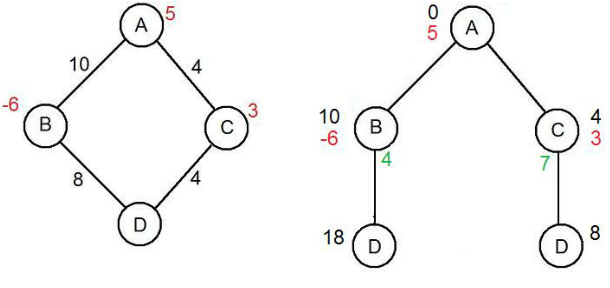
\includegraphics[width=0.75\columnwidth]{aufgabe5f}
\end{figure}


An diesem Beispiel kann man sehen, dass wenn man den Algorithmus durchf\"uhren m\"ochte, um einen k\"urzesten Weg von D nach A zu finden, man alle beiden Wege \"uberpr\"ufen wird. Allerdings w\"urde man dies nicht tun, wenn statt -6 als heuristischer Wert 0 eingesetzt werden w\"urde, da der Gesamtwert nicht mehr 4 sondern 10 w\"are und somit in Anbetracht der Gesamtkosten des Pfades A-C-D gar nicht gepr\"uft werden m\"usste. Bei gr\"o{\ss}eren Beispielen kann dies zu erheblichen Teilpfaden f\"uhren, die man weglassen k\"onnte und somit effektiver arbeiten.

\subsection*{5.g)}
Die Vollst\"andigkeit des Algorithmus ist weiterhin gegeben, da wenn ein Pfad nicht zu einem Zielknoten f\"ihrt, ein anderer gepr\"uft werden w\"urde und dies so lange bis mindestens ein Punkt erreicht wird an dem Start- und Zielknoten wie gew\"unscht sind. Sollte kein
derartiger Pfad existieren, kann der Algorithmus keinen Pfad finden und von daher kann man solche F\"alle vernachl\"assigen.

Die Optimalit\"at wird ebenfalls nicht beeintr\"achtigt, da die heuristische Werte nur Sch\"atzwerte sind, die ein schnelleres Finden des besten Weges erm\"oglichen sollen. Wenn wir negative heuristische Werte zulassen, finden wir den gew\"unschten Weg evtl. nicht schneller, aber solange wir Heuristiken benutzen, die die tats"achlichen Kosten untersch\"atzen, erreichen wir trotzdem die beste L\"osung.

Dies gilt, weil f\"ur die Gesamtkosten der Wege am Ende die heuristischen Werte keinen Einfluss haben. Die \"Uberpr\"ufung anderer - vielleicht besserer - Wege wird gew\"ahrleistet durch die Untersch\"atzung, denn somit wird kein potenzieller Weg durch die heuristischen Werte als "`nicht weiter zu \"uberpr\"ufen"' gekennzeichnet.

\section*{Aufgabe 6}
\subsection*{6.a)}
w=weiß, g=grau, s=schwarz\\
\begin{tabular}{|c | c | c |c | c | c |}
\hline
  Schritt & A & B & C & D & E \\
  \hline
\hline
Startbelegung &  w & w  & w & w  & w  \\

Startkonflikte(10) &  w(10)g(7)s(7) & w(10)\textbf{g(6)},s(6)  & w(10)g(7)s(7) & w(10)g(7)s(7)  & w(10)g(7)s(7)  \\
  \hline
      1 &  w & g  & w & w  & w  \\

  (6)&  w(6)g(5)\textbf{s(4)} & w(10)g(6),s(6)  & w(6)g(5)s(4) &w(6)g(5)s(4)&w(6)g(5)s(4)  \\
  \hline
    2 &  s & g  & w & w  & w  \\

   (4)&  w(6)g(5)s(4) & w(7)g(4)s(5)  & w(4)g(3)\textbf{s(2)} &w(4)g(4)s(4)&w(4)g(3)s(2)  \\
    \hline
  3 &  s & g  & s & w  & w  \\
   (2)& w(4)g(3)s(2) & w(4)g(2)s(3) & w(4)g(3)s(2) &w(2)g(2)s(2)  &w(2)g(2)s(2)   \\
    \hline
  4 &  s & g  & s & w  & w  \\
   (1)& w(2)g(2)s(1)  & w(3)g(1)s(3)  & w(2)g(2)s(1) & w(1)g(1)s(1) & w(1)g(1)s(1) \\
    \hline
 \end{tabular}\\ 
 \begin{tabular}{|c | c | c |}
 \hline
   Schritt & F & G \\
   \hline
 \hline
     Startbelegung &  w & w \\
   Startkonflikte(10) &  w(10)g(8)s(8) & w(10)g(8)s(8)\\
   \hline
   1 &  w & w \\
    (6)&  w(6)g(4)s(4) & w(6)g(4)s(4)  \\
     \hline
   2 &  w & w \\
    (4)&  w(4)g(3)s(4) & w(4)g(2)s(2)  \\
     \hline
   3 &  w & w \\
    (2)&  w(2)\textbf{g(1)}s(2) & w(2)g(1)s(2)  \\
     \hline
   4 &  g & w \\
    (1)&  w(2)g(1)s(2) & w(1)g(2)s(2)  \\
     \hline
  \end{tabular}\\
  
  
  Das Ergebnis hat immer noch einen Konflikt, d.h. der Algorithmus ist zu keiner Lösung gekommen.
  
\subsection*{6.b)}
Die Tie-Break-Regel muss dahingehend ge\"andert werden, dass sie den den höchsten lexikographischen Folgezustand bevorzugt.\\
\\
In 6.a) ist das Problem, dass sehr fr\"uh A und C belegt werden. Dann ist aber D durch A und B festgelegt und E ist durch B und C festgelegt. Die Constraintverletzung zwischen D und E kann dann nicht mehr in einem Schritt gel\"ost werden und die lokale Suche bleibt somit in einem lokalen Minimum stecken.

Die ge\"anderte Tie-Break-Regel belegt nun hingegen A und C sp\"ater und daf\"ur E fr\"uher. Somit kommt es zu keinem Konflikt zwischen D und E. Die sp\"atere Belegung von A und C f\"uhrt zu keinen Problemen, denn deren Konflikte mit F bzw. G k\"onnen immer in einem Schritt gel\"ost werden, da F und G nur zwei Constraints haben.

\end{document}
